% L13c figure: why a standard cuts the connection code.
%
% Two panels with the same three applications and four programs that offer
% tools. Without a standard (left), each application needs its own connection
% code for each program: 3 x 4 = 12 lines. With MCP (right), each application
% and each program implements the protocol once: 3 + 4 = 7 lines into one MCP
% box. The figure follows the MCP definition in the Language Models and Tools
% section.
%
% Drawn on November 18, 2026 with the palette and build of the other L13c
% figures. The notebook SVG carries a dark palette added by theme_svg.py; keep
% new colors in that script's mapping when changing the palette here.
\documentclass[tikz,border=4pt]{standalone}
\usepackage[no-math]{fontspec}
\IfFontExistsTF{Arial}{\setsansfont{Arial}}{\setsansfont{TeX Gyre Heros}}
\renewcommand{\familydefault}{\sfdefault}
\usetikzlibrary{arrows.meta, calc}

% Ink, blue, gray, and band match the other L13c figures. Blue marks MCP.
\definecolor{vnink}{HTML}{202124}
\definecolor{gdblue}{HTML}{0091FF}
\definecolor{gdgray}{HTML}{6D7278}
\definecolor{waband}{HTML}{EEF0F2}

\begin{document}
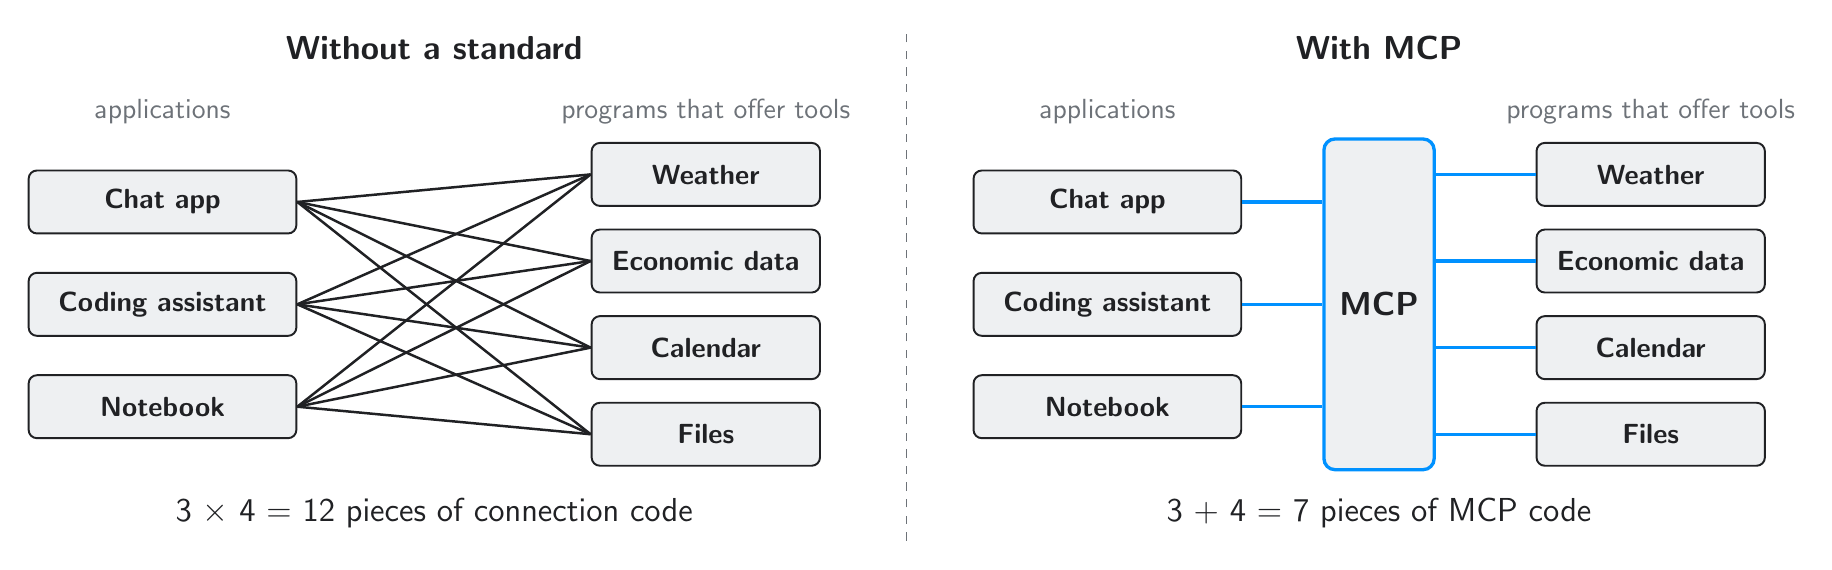
\begin{tikzpicture}[
  font=\sffamily\large,
  box/.style={draw=vnink, rounded corners=3pt, minimum height=0.8cm,
    fill=waband, line width=0.7pt, text=vnink, align=center,
    font=\sffamily\normalsize\bfseries},
  app/.style={box, minimum width=3.4cm},
  program/.style={box, minimum width=2.9cm},
  title/.style={font=\sffamily\large\bfseries, text=vnink},
  column/.style={font=\sffamily\normalsize, text=gdgray},
  count/.style={font=\sffamily\large, text=vnink},
  code/.style={line width=0.9pt, draw=vnink},
  mcp/.style={line width=1.2pt, draw=gdblue}
]

% The same applications and programs in both panels. Each panel is shifted by \dx.
\foreach \dx/\panel in {0/left, 12.0/right} {
  \begin{scope}[shift={(\dx, 0)}]
    \node[app] (\panel-app1) at (1.5, 2.80) {Chat app};
    \node[app] (\panel-app2) at (1.5, 1.50) {Coding assistant};
    \node[app] (\panel-app3) at (1.5, 0.20) {Notebook};
    \node[program] (\panel-prog1) at (8.4, 3.15) {Weather};
    \node[program] (\panel-prog2) at (8.4, 2.05) {Economic data};
    \node[program] (\panel-prog3) at (8.4, 0.95) {Calendar};
    \node[program] (\panel-prog4) at (8.4, -0.15) {Files};
    \node[column] at (1.5, 3.95) {applications};
    \node[column] at (8.4, 3.95) {programs that offer tools};
  \end{scope}
}

% ------------------------------------------- left: one piece of code per pair
\foreach \a in {1, 2, 3} {
  \foreach \p in {1, 2, 3, 4} {
    \draw[code] (left-app\a.east) -- (left-prog\p.west);
  }
}
\node[title] at (4.95, 4.75) {Without a standard};
\node[count] at (4.95, -1.15) {3 $\times$ 4 = 12 pieces of connection code};

% ------------------------------------------ right: one implementation per box
\node[draw=gdblue, rounded corners=4pt, line width=1.2pt, fill=waband,
  minimum width=1.4cm, minimum height=4.2cm, text=vnink,
  font=\sffamily\large\bfseries] (protocol) at (16.95, 1.50) {MCP};
\foreach \a in {1, 2, 3} {
  \draw[mcp] (right-app\a.east) -- (right-app\a.east -| protocol.west);
}
\foreach \p in {1, 2, 3, 4} {
  \draw[mcp] (right-prog\p.west -| protocol.east) -- (right-prog\p.west);
}
\node[title] at (16.95, 4.75) {With MCP};
\node[count] at (16.95, -1.15) {3 + 4 = 7 pieces of MCP code};

% a thin divider between the two panels
\draw[gdgray, line width=0.6pt, dash pattern=on 3pt off 3pt] (10.95, -1.5) -- (10.95, 5.0);

\end{tikzpicture}
\end{document}
